% Chapter 1

\chapter{The current state of the subject.} % Main chapter title
\label{Chapter1} % For referencing the chapter elsewhere, use \ref{Chapter1} 
\lhead{Chapter 1. \emph{The current state of the subject}} % This is for the header on each page - perhaps a shortened title

\iffalse
Doposiaľ používané metódy pre analýzu elektrofyzikálnych vlastností
štruktúry MOS sú založené na predpoklade, že jej substrát má homogénnu
dotáciu prímesí. Táto problematika bola riešená na Katedre
mikroelektroniky v rámci štátnych výskumných úloh \cite{1.1,1.2} a v
kandidátskych dizertačných prácach \cite{1.5,1.6,1.7,1.8}. Tieto práce
poskytujú potrebný prehľad o riešení uvedenej problematiky vo svete a
tiež na našom pracovisku. Keďže v súčasnosti sa pri výrobe
unipolárnych integrovaných obvodov využíva iónová implantácia pre
riadenie elektrických vlastností integrovaných súčiastok, je žiadúce
pre ovládanie vlastností polovodičových štruktúr poznať parametre
štruktúr MOS s nehomogénnou dotáciou substrátu. Pre tieto účely bola
výskumná úloha {\em Elektrofyzikálne vlastnosti mikroelektronických
štruktúr} \cite{1.3,1.4} zameraná na vývoj diagnostických metód pre
výskum vlastností technologických procesov pomocou štruktúr MOS s
nehomogénnou dotáciou prímesí a ich aplikáciu na riešenie problémov
Česko-Slovenského polovodičového priemyslu. Z tohoto zamerania štátnej
výskumnej úlohy vychádza aj zameranie predloženej kandidátskej
dizertačnej práce. Potreba riešiť tento problém vychádza aj zo
skutočnosti, že dosiaľ sa u nás touto problematikou, pokiaľ je nám
známe, nikto nezaoberal. Naviac sa problematika rozšírila aj na výskum
homogenity rozloženia elektrofyzikálnych parametrov štruktúr MOS na
kremíkovom substráte, ktorá je mimoriadne závažná aj z hľadiska
zvýšenia kvality procesu vytvárania polovodičových štruktúr a
integrovaných obvodov planárnou technológiou. Na základe
predchádzajúcich skutočností uvedieme v ďalšej časti tejto kapitoly
len najnutnejšie poznatky, ktoré sú potrebné pre riešenie danej
problematiky.
\fi

Up to now, the methods used for analysis of electrophysical properties
of MOS structures are based on the assumption that the distribution of
impurities in the substrate is homogeneous. This issue was addressed
by the Department of Microelectronics within the goverment research
projects \cite{1.1,1.2} and PhD thesis \cite{1.5,1.6,1.7,1.8}. These
works provide the necessary overview of the solutions for the problems
globaly and also in our department. Whereas at present in the
manufacture of unipolar integrated circuits using ion implantation for
control the electrical properties of integrated components, it is
desirable to control the properties of semiconductor structures to
know the parameters of MOS structures with inhomogeneous subsidy
substrate. For this purpose was research task {\em Electrophysical
  properties of microelectronic structures} \cite{1.3,1.4} focused on
the development of diagnostic methods for study of the properties of
technological processes using MOS structures with inhomogeneous
subsidy impurities and their application to solving problems of
Czech-Slovak semiconductor industry. From this target of the goverment
research project resulted the focus of the presented thesis. The need
to address this issue is also based on the fact that up till now this
issue, as far as we known, has never been studied here. Additionally,
the issue was extended to the research of electro-physical parameters'
homogeneity of MOS structures on silicon substrate, which is
particularly serious in the light of the process quality improvement
of forming a semiconductor structures and integrated circuits by
planar technology. Based on the foregoing, we list later in this
chapter only the most necessary knowledge needed to deal with the
issues.

\section{Základné poznatky o štruktúre MOS.}

Štruktúra MOS tvorí jednoduchú testovaciu štruktúru, ktorej meraním
možno skúmať skoro všetky jej elektrické vlastnosti. Výhodnosť
štruktúry MOS spočíva v jednoduchosti jej výroby a jednoduchosti
analýzy jej vlastností. Jednoduchosť analýzy vyplýva z toho, že
analyzovaný systém je v tepelnej rovnováhe a zároveň
jednodimenzionálny prístup je pre väčšinu javov dostatočne
presný. Elektrickými meraniami štruktúry MOS možno skúmať vlastnosti
objemu $SiO_2$, jeho rozhrania s polovodičom a kovom, ako aj
vlastnosti podpovrchovej oblasti polovodiča.

\section{Ideálna štruktúra MOS.}  \index{MOS!ideálna štruktúra}

Štruktúru MOS možno považovať za dvojpól, ktorého náhradnú schému si
možno predstaviť ako sériové zapojenie napäťovonezávislej kapacity
oxidu $C_{ox}$ a kapacity oblasti priestorového náboja (OPN)
$C_{sc}(\varphi_{s})$, ktorá je funkciou povrchového potenciálu
polovodiča. Potom pre kapacitu štruktúry MOS platí \cite{I.1}

\begin{equation}\label{eq:1.1}
\frac{1}{C_{mos}(V_g)} = \frac{1}{C_{ox}} + \frac{1}{C_{sc}(\varphi_s)}
\end{equation}

Pri analýze štruktúry MOS sa používajú následovné zjednodušujúce
predpoklady, ktoré definujú ideálnu štruktúru MOS:

\begin{itemize}
\item hustota pascí rozhrania $Si-SiO_2$ je rovná nule 
\item v izolátore, ktorý tvorí $SiO_2$, sa nenachádzajú náboje 
\item rozdiel výstupných potenciálov z kovu a polovodiča je rovný nule
\item platí vzťah $V_{g}=V_{ox}+\varphi_{s}$  .
\end{itemize}

\noindent V závislosti od hradlového napätia možno rozlíšiť tieto
pracovné režimy štruktúry MOS:

\begin{itemize}
\item režim obohatenia
\item stav vyrovnaných pásov
\item režim ochudobnenia a inverzie (hlbokého ochudobnenia).
\end{itemize}

\section{Kapacitné závislosti ideálnej štruktúry MOS.}

Pre všetky uvedené prípady platí v polovodiči jednodimenzionálna
Poissonova rovnica

\begin{equation}\label{eq:1.2}
\frac{d^2\varphi}{dx^2}=-\frac{q}{\varepsilon}(p-n+N_{p}-N_{A})
\end{equation}
\index{Poissonova rovnica}

ktorá určuje priebeh elektrického potenciálu $\varphi$ ako funkciu
vzdialenosti od povrchu polovodiča $x$. Rovnicu \ref{eq:1.2} možno
analyticky vyriešiť len pre určité špeciálne prípady priebehu
koncentrácie prímesí a vo všeobecnosti treba použiť numerické metódy
\cite{1.9,1.10}. Potom pre známy priebeh koncentrácie prímesí v
polovodiči možno získať priebeh elektrického potenciálu v polovodiči,
pričom napätie hradla považujeme za parameter, určujúci stav
štruktúry. Pre bližšie ozrejmenie fyzikálnych procesov v štruktúre MOS
pri prechode zo stavu akumulácie do inverzie, alebo hlbokého
ochudobnenia sme riešili rovnicu \ref{eq:1.2}, kde pri vhodnej
variácii parametra $V_g$ možno zároveň získať priebeh povrchového
potenciálu ako funkciu napätia hradla $\varphi_{s}(V_g)$ a závislosť
kapacity štruktúry MOS $C_{mos}(V_g)$ (Dodatok \ref{app:AppendixA}).

\begin{figure}[h!]\centering
%\framebox[10cm]{\rule{0cm}{3cm}}
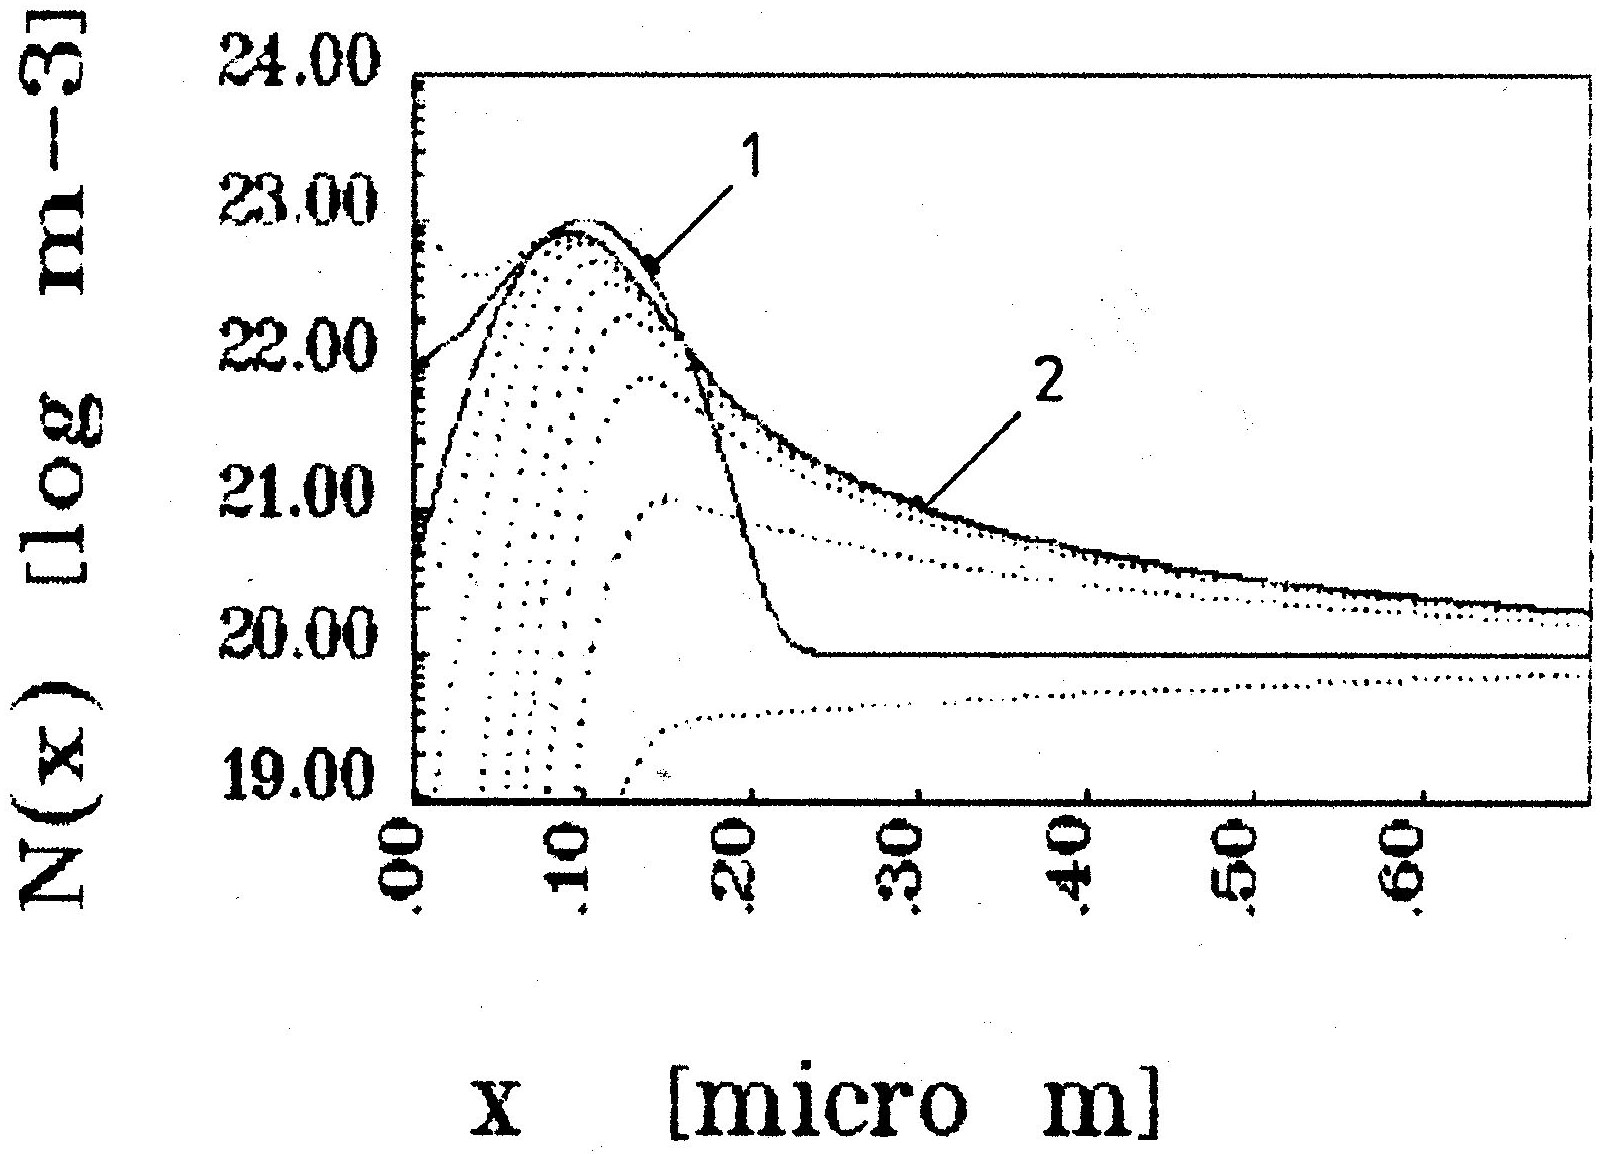
\includegraphics{Figures/fig-1-1.eps}
\captionsetup{justification=raggedright, singlelinecheck=false}
\caption[Priebeh koncentrácie prímesí v podpovrchovej oblasti
  polovodiča]{Priebeh koncentrácie prímesí v podpovrchovej oblasti
  polovodiča simulovaný Gaussovským rozložením \cite{1.11} s
  následovnými parametrami $R_p=0.1 \mu{m}$; $\Delta{R_p}=0.03
  \mu{m}$; $N_{max}=10^{23} m^{-3}$; $N_{bulk}=10^{20} m^{-3}$
  (označený plnou čiarou 1). Priebeh majoritných nosičov náboja pre
  $V_g=0$ (označený plnou čiarou 2). Bodkovanými čiarami sú znázornené
  priebehy koncentrácií majoritných nosičov pre napätia hradla rôzne
  od nuly. Stav termodynamickej rovnováhy medzi rozložením prímesí a
  nosičov náboja je popísaný v dodatku \ref{app:AppendixD}.}
\label{fig:1.1}
\end{figure}

\par Na obrázku \ref{fig:1.1} je znázornený priebeh koncentrácie
prímesí v polovodiči (simulovaný Gaussovským priebehom) a priebehy
majoritných nosičov náboja pre stav štruktúry meniaci sa od obohatenia
do inverzie, znázorňujúce dej ochudobňovania podpovrchovej oblasti
polovodiča. Tu vidieť, že priebeh koncentrácie majoritných nosičov v
implantovanej oblasti nadobúda maximum a potom klesá ku koncentrácii
substrátu, ktorú dosiahne v bode nulového elektrického potenciálu.
Zároveň je zrejmý rozdiel medzi priebehom koncentrácie prímesí a
priebehom koncentrácie majoritných nosičov náboja v stave
termodynamickej rovnováhy pre nulové napätie hradla, ktorý vzniká v
dôsledku difúzie majoritných nosičov náboja.

\begin{figure}[h!]\centering
%\framebox[10cm]{\rule{0cm}{3cm}}
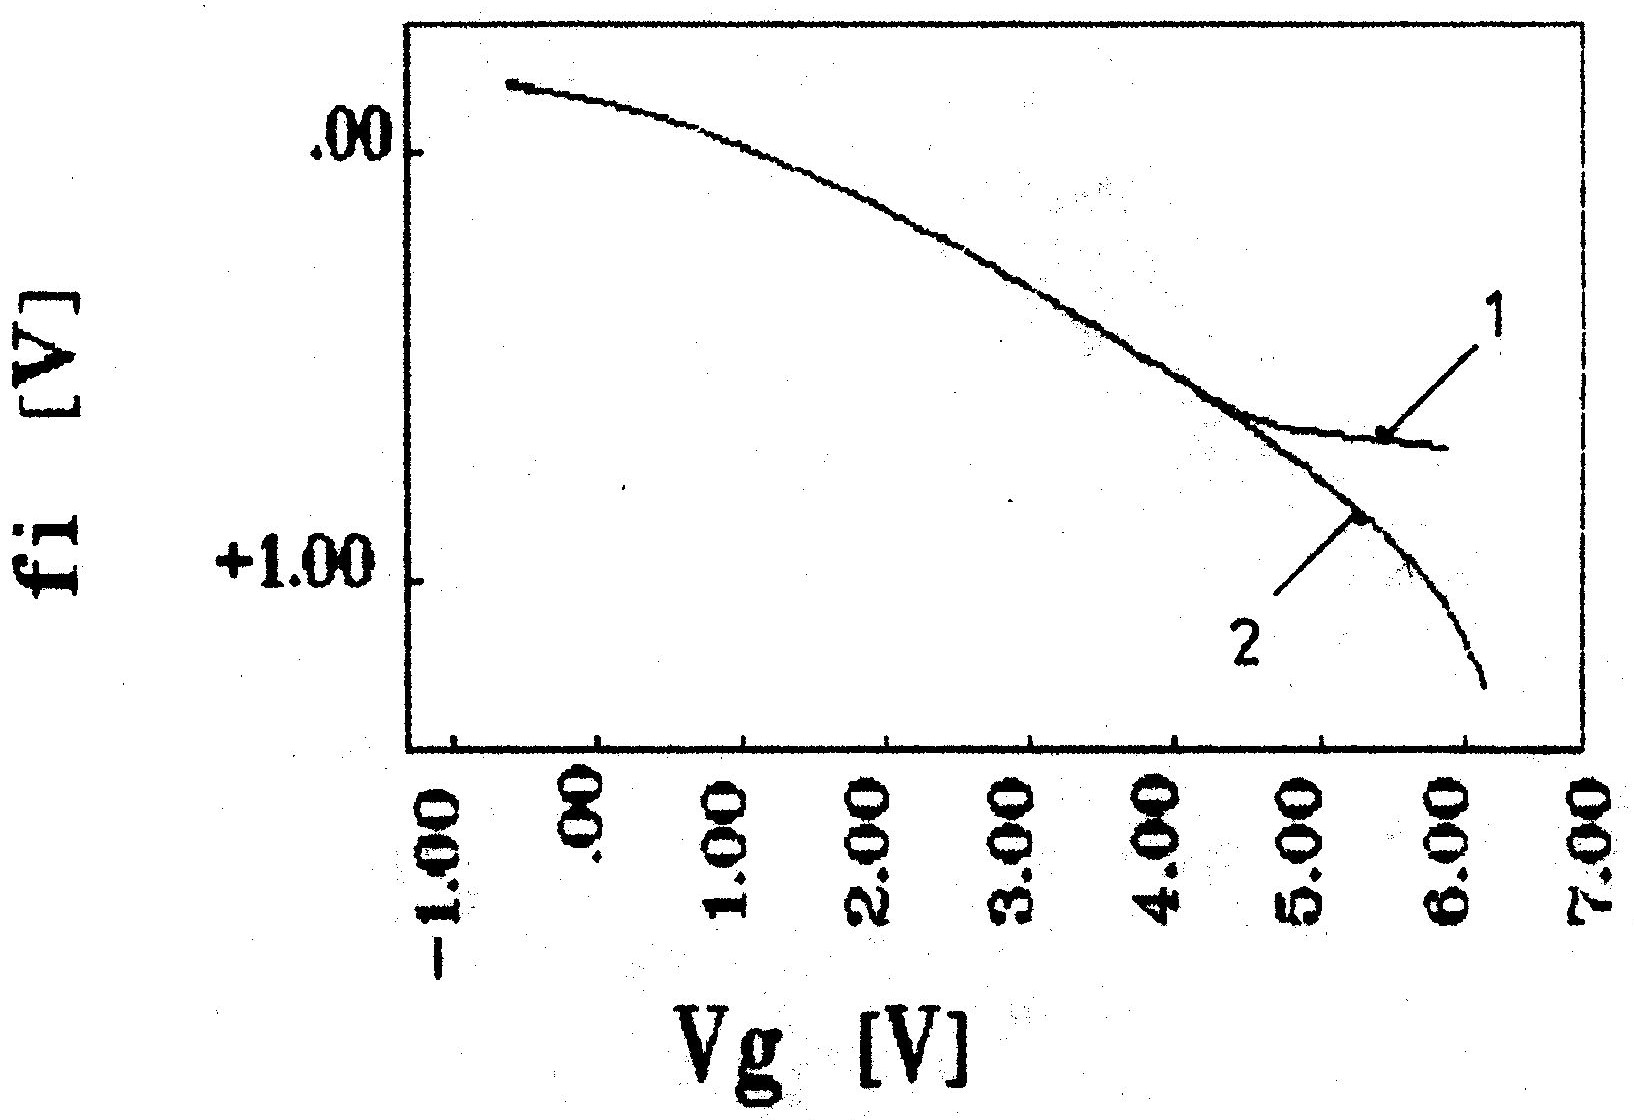
\includegraphics{Figures/fig-1-2.eps}
\captionsetup{justification=raggedright, singlelinecheck=false}
\caption[Priebeh povrchového potenciálu $\varphi_s(V_g)$ ako funkcie
  napätia hradla]{Priebeh povrchového potenciálu $\varphi_s(V_g)$ ako
  funkcie napätia hradla pre nízkofrekvenčné (LF) a vysokofrekvenčné
  (HF) meranie (označený 1) a pre meranie v stave hlbokého
  ochudobnenia (označený 2).}
\label{fig:1.2}
\end{figure}

\par Na obrázku \ref{fig:1.2} sú znázornené priebehy povrchového
potenciálu pre rôzne režimy merania štruktúry MOS. V oblasti
obohatenia a ochudobnenia sú obidva priebehy rovnaké. Od počiatku
inverzie sa povrchový potenciál pre LF a HF meranie ustaľuje v
dôsledku vytvárania inverznej vrstvy.  Krivka hlbokého ochudobnenia
ďalej klesá. Tento stav sa v reálnej štruktúre ukončí elektrickým
prierazom.

\par Na obrázku \ref{fig:1.3} sú znázornené kapacitne-napäťové
závislosti štruktúry MOS. Všetky tri krivky majú spoločný priebeh v
oblasti obohatenia a ochudobnenia (spoločný priebeh majú aj krivky
povrchového potenciálu). V tejto časti klesá kapacita pomaly, pretože
oblasť priestorového náboja sa rozpína cez oblasť s vysokou
koncentráciou prímesí (obr.1.1). Od počiatku inverzie sa krivky
rozdeľujú. Nízkofrekvenčná krivka, ktorá zaznamenáva inverznú vrstvu,
stúpa až ku kapacite oxidu. Vysokofrekvenčná krivka nezaznamenáva
inverznú vrstvu, pretože minoritné nosiče nestačia sledovať
vysokofrekvenčný merací signál, avšak kapacita už ďalej neklesá,
pretože so zvyšovaním napätia hradla sa zvyšuje prevážne koncentrácia
minoritných nosičov v inverznej vrstve a oblasť priestorového náboja
sa ďalej nerozpína.

\begin{figure}[h!]\centering
%\framebox[10cm]{\rule{0cm}{3cm}}
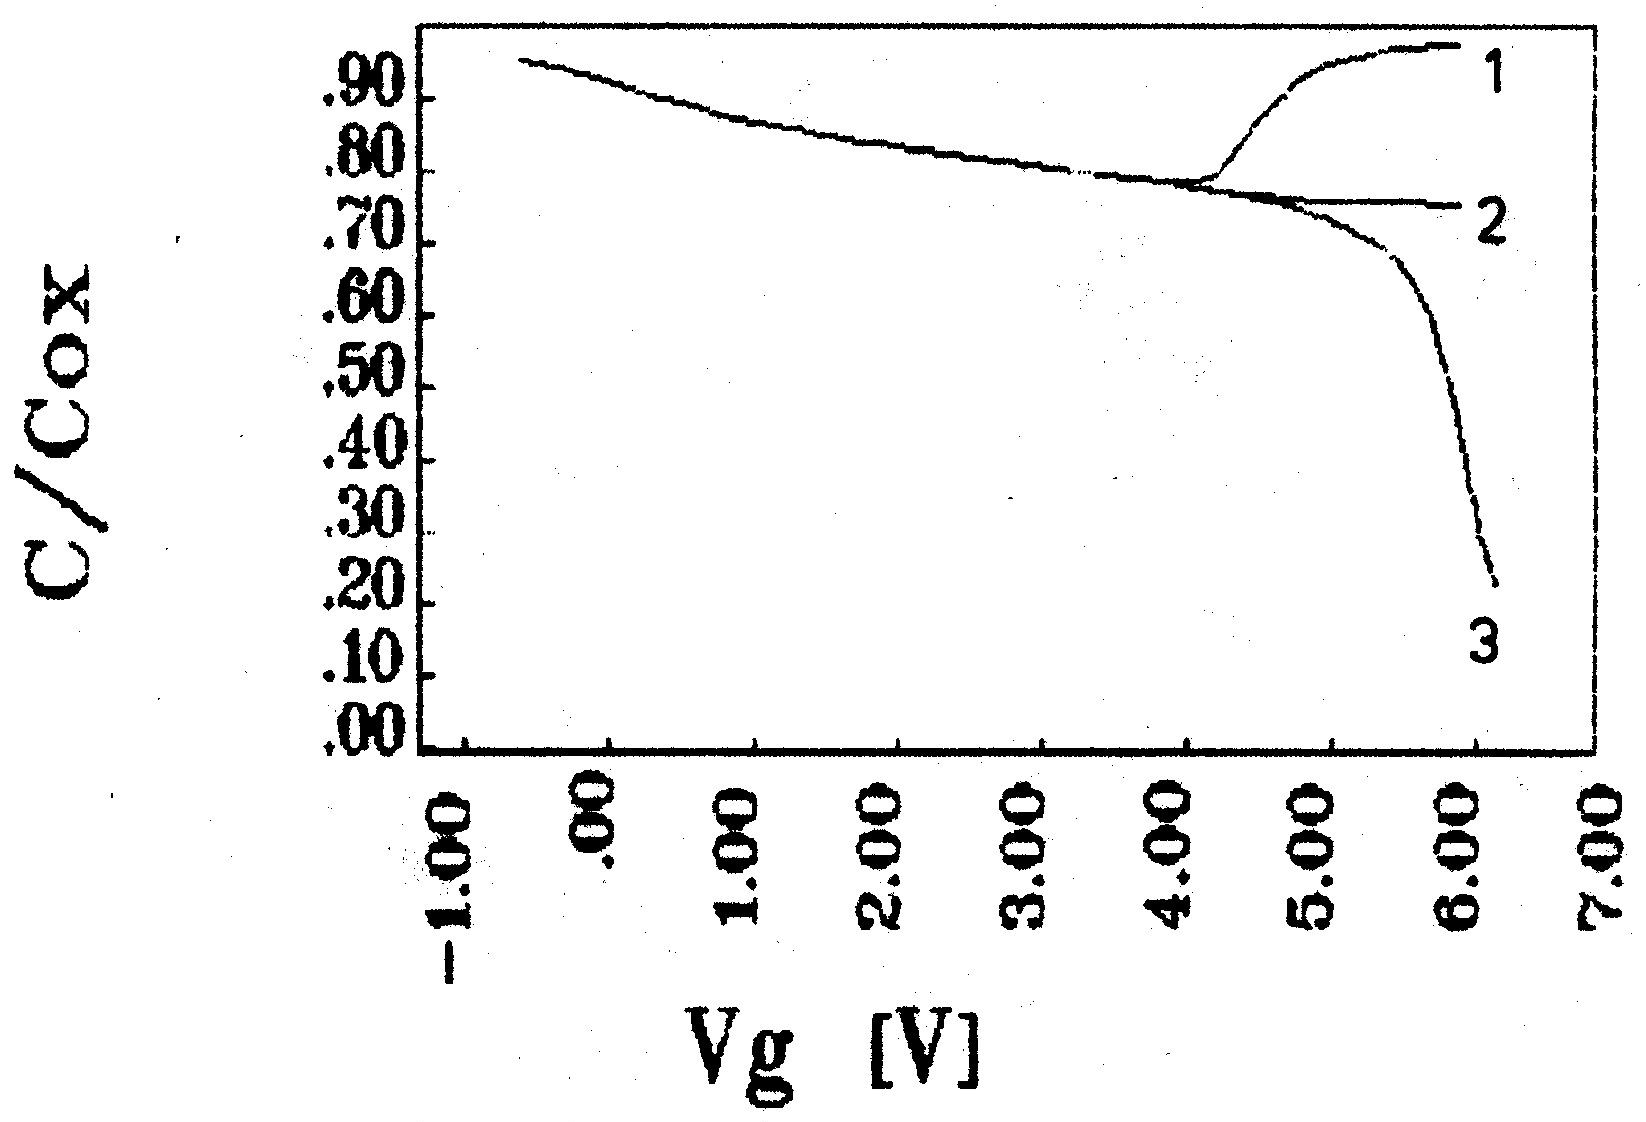
\includegraphics{Figures/fig-1-3.eps}
\captionsetup{justification=raggedright, singlelinecheck=false}
\caption[Priebeh kapacity štruktúry MOS v závislosti od napätia
  hradla]{Priebeh kapacity štruktúry MOS v závislosti od napätia
  hradla pre nízkofrekvenčné meranie (označené 1), vysokofrekvenčné
  meranie (označené 2) a meranie v stave hlbokého ochudobnenia
  (označené 3).}
\label{fig:1.3}
\end{figure}

\par V stave hlbokého ochudobnenia sa nevytvára inverzná vrstva a so
zvyšovaním napätia hradla sa oblasť priestorového náboja naďalej
rozpína a kapacita klesá. Z obrázku \ref{fig:1.3} je vidieť, že po
prekonaní oblasti s vysokou koncentráciou prímesí krivka hlbokého
ochudobnenia začína klesať rýchlejšie.

\section{Reálna štruktúra MOS.}  Odlišnosť ideálnej a reálnej
štruktúry MOS bola obsažne spracovaná v práci \cite{1.12} a tu
uvedieme len prehľad tejto problematiky. Elektrické vlastnosti reálnej
štruktúry MOS sa líšia od ideálneho modelu hlavne vplyvom poruchových
nábojov v oxidovej vrstve a na jej rozhraní s polovodičom a kovom,
ktoré možno rozdeliť do nasledovných skupín:

\begin{itemize}
\item náboj pohyblivých iónov vo vrstve oxidu - $Q_{m}$
\item náboj ionizovaných pascí v oxide - $Q_{ox}$
\item fixný náboj na rozhraní $Si-SiO_2$ , spôsobený nestechiometrickým
  zložením v oblasti fázového prechodu - $Q_f$
\item náboj pascí na rozhraní $Si-SiO_2$  - $Q_{it}$
\end{itemize}

\par Zároveň na elektrické vlastnosti štruktúry MOS vplýva aj rozdiel
výstupných potenciálov elektrónov z kovu a polovodiča,
$\varphi_{ms}\neq{0}$.  Okrem uvedených poruchových nábojov na
elektrické vlastnosti štruktúry MOS vplývajú aj geometrické
nedokonalosti štruktúry, ako aj zmena hrúbky izolačnej vrstvy a
nerovinnosť plochy rozhrania $Si-SiO_2$ . Pri prechode k veľmi veľkej
integrácii vznikla potreba zaoberať sa aj mikrodefektami v objeme
kremíka, ktoré predstavujú poruchy kryštalickej mriežky pri výrobe
monokryštálu, jeho primárnom spracovaní do formy kremíkového plátku a
v priebehu technologického spracovania súčiastky. Ak sa uvedené
defekty nachádzajú vo funkčnej oblasti súčiastky, majú nepriaznivé
účinky na elektrické parametre, avšak v objeme polovodiča mikrodefekty
vhodných veľkostí spôsobujú getračné efekty, čo sa často využíva na
tvorbu tzv. denudovanej zóny.  Zámerným vytváraním mikrodefektov v
objeme polovodiča pomocou implantácie uhlíka a následným tepelným
spracovaním možno napríklad podstatne zvýšiť dobu života minoritných
nosičov náboja \cite{1.13}. V práci \cite{1.14} autori zreteľne
zobrazili pomocou laserovej rastrovacej tomografie denudovanú zónu pri
povrchu kremíka, vytvorenú getračnými efektami mikroprecipitátov
$SiO_x$. Zároveň je z obrázkov vidieť mikroprecipitáty v objeme
polovodiča, vytvorené pomocou kyslíka a patričného tepelného
spracovania.

\begin{thebibliography}{}
\bibitem[1.1]{1.1} Csabay O. et al: Výskum štruktúr MIS a
  pasivácie. Záverečná správa štátnej výskumnej úlohy III-4-3/2. EF
  SVŠT, Bratislava 1980.
\bibitem[1.2]{1.2} Csabay O. et al: Výskum elektrofyzikálnych
  vlastností mikroelektronických unipolárnych štruktúr. Záverečná
  správa štátnej výskumnej úlohy III-6-1/13. EF SVŠT, Bratislava 1985.
\bibitem[1.3]{1.3} Csabay O., Botka V. et al: Elektrofyzikálne
  vlastnosti mikroelektronických štruktúr. Priebežná správa Štátnej
  výskumnej úlohy III-7-2/04. Katedra mikroelektroniky EF SVŠT,
  Bratislava 1988.
\bibitem[1.4]{1.4} Csabay O., Botka V. et al: Elektrofyzikálne
  vlastnosti mikroelektronických štruktúr. Záverečná správa Štátnej
  výskumnej úlohy III-7-2/04, Katedra mikroelektroniky EF SVŠT,
  Bratislava 1990.
\bibitem[1.5]{1.5} Žiska M.: Kandidátska dizertačná práca. Katedra
  mikroelektroniky EF SVŠT, Bratislava 1985.
\bibitem[1.6]{1.6} Harmatha L.: Výskum vlastností štruktúry MIS v
  nerovnovážnom stave kapacitnou metódou. Kandidátska dizertačná
  práca. Katedra mikroelektroniky EF SVŠT, Bratislava 1983.
\bibitem[1.7]{1.7} Valehrachová D.: Kandidátska dizertačná
  práca. Katedra mikroelektroniky EF SVŠT, Bratislava
\bibitem[1.8]{1.8} Kinder R.: Príspevok ku skúmaniu koncentračných
  profilov implantovaných vrstiev. Kandidátska dizertačná práca. EF
  SVŠT Bratislava 1984.
\bibitem[1.9]{1.9}
El- Sissi H., Cobbold R.S.C.: Electronic Letters 25 (1973) s.594.
\bibitem[1.10]{1.10} Klopfenstein R. W., Wu Chung P.: IEEE Trans. on
  electron. devices ED-22 (1975) s.329.
\bibitem[1.11]{1.11}
Ryssel H., Ruge I.: Ionenimplantation. Stuttgart 1978
\bibitem[1.12]{1.12} Csabay O.: Niektoré technologické a fyzikálne
  problémy štruktúr MIS. Doktorská dizertačná práca. Katedra
  mikroelektroniky, EF SVŠT, Bratislava 1986.
\bibitem[1.13]{1.13}
Skorupa W., Kogler R. : Electronics Letters Vol.25 (1989) s.1898.
\bibitem[1.14]{1.14}
Gall P. at al. : Electronics Letters Vol.25 (1989) s.429
\end{thebibliography}
